\documentclass{article}


% if you need to pass options to natbib, use, e.g.:
%     \PassOptionsToPackage{numbers, compress}{natbib}
% before loading neurips_2022

% ready for submission
\usepackage[preprint]{neurips_2022}
\PassOptionsToPackage{square,numbers}{natbib}
%\usepackage[square,numbers]{natbib}


% to compile a preprint version, e.g., for submission to arXiv, add add the
% [preprint] option:
%     \usepackage[preprint]{neurips_2022}


% to compile a camera-ready version, add the [final] option, e.g.:
%     \usepackage[final]{neurips_2022}


% to avoid loading the natbib package, add option nonatbib:
%    \usepackage[nonatbib]{neurips_2022}


\usepackage[utf8]{inputenc} % allow utf-8 input
\usepackage[T1]{fontenc}    % use 8-bit T1 fonts
\usepackage{hyperref}       % hyperlinks
\usepackage{url}            % simple URL typesetting
\usepackage{booktabs}       % professional-quality tables
\usepackage{amsfonts}       % blackboard math symbols
\usepackage{nicefrac}       % compact symbols for 1/2, etc.
\usepackage{microtype}      % microtypography
\usepackage{xcolor}         % colors
\usepackage{graphicx}


\title{Machine Learning Approach to Predict Diabetes Complications}


% The \author macro works with any number of authors. There are two commands
% used to separate the names and addresses of multiple authors: \And and \AND.
%
% Using \And between authors leaves it to LaTeX to determine where to break the
% lines. Using \AND forces a line break at that point. So, if LaTeX puts 3 of 4
% authors names on the first line, and the last on the second line, try using
% \AND instead of \And before the third author name.


\author{%
  Muhammad Aji Muharrom %\thanks{Use footnote for providing further information
    %about author (webpage, alternative address)---\emph{not} for acknowledging
    %funding agencies.} \\
  %Department of Computer Science\\
  %Cranberry-Lemon University\\
  %Pittsburgh, PA 15213 \\
  \texttt{ajimuharrom@uchicago.edu} \\
  % examples of more authors
  % \And
  % Coauthor \\
  % Affiliation \\
  % Address \\
  % \texttt{email} \\
  % \AND
  % Coauthor \\
  % Affiliation \\
  % Address \\
  % \texttt{email} \\
  % \And
  % Coauthor \\
  % Affiliation \\
  % Address \\
  % \texttt{email} \\
  % \And
  % Coauthor \\
  % Affiliation \\
  % Address \\
  % \texttt{email} \\
}


\begin{document}


\maketitle


\begin{abstract}
  The global burden of diabetes mellitus (DM) is expected to increase, reaching 590 million people in 2035. Uncontrolled DM leads to various complications with devastating consequences for patients and burdens the health system. Early identification of individuals at risk in developing these complications might benefit to provide targeted intervention. Machine learning models to predict 3-year risk of complications were developed for diabetes patients using 2 years worth of recorded data in the healthcare system on a realistic synthetic dataset. Best overall performance on the testing dataset was 80.2\% overall accuracy using the ordinary least squares method. The support vector machine classifier was able to perform decently in training but did not generalize well in testing, with best performance of 72.4\% accuracy. 
\end{abstract}


\section{Introduction}

Diabetes mellitus (DM) is one of the most common endocrine disorder, with global burden projected to increase from 380 million people in 2013 to 590 million in 2035.\cite{kavakiotis,ravaut21}  It is also among the top 3 reasons of primary care provider visits in the US.\cite{synthea} Uncontrolled DM causes chronic hyperglycemia, which is linked to several complications with devastating consequences leading to permanent morbidity and mortality. Therefore, it is of high importance for diabetic patients to receive appropriate care to maintain normal blood glucose levels and prevent further complications. Early identification of individuals at risk in developing these complications is substantial for better targeted interventions that could further prevent and lower incidences of these conditions.\cite{ravaut21}

% \label{heading}
% \ref{heading}

\section{Methods}

\subsection{Project Description}

The goal of this project is to develop a model predictive of diabetes complications among cohort of diabetic patients using longitudinal time-series data. The model receives 2 years worth of medical data as input and predicts occurence of diabetes complication in the next 3 years.

\subsection{Dataset}

Dataset for this project were synthetic medical record data generated by Synthea, a well-known tool for generating realistic but unreal medical data.[paper] The dataset was generated using default options, with a slight modification to produce csv files as output with at least 50,000 living individuals. Following this, health record on 8 different tables were generated. The resulting dataset represents the health condition of Massachusetts healthcare consumers, containing more than 58,000 individuals with comprehensive medical record including birth-to-death entire lifecycle and course of specific medical conditions. Generated tables include: (1) the Patients table, which includes patients' date of birth, gender, race, and date of death if applicable; (2) the Observations table, which stores every medical data observations of the patients that has been recorded in the health system; (3) Conditions table, which documents medical conditions and diagnoses of the patients as recorded in the health system; (4) Medications table, which records every medications dispensed to every patient in the health system. All medical-related concepts included were also encoded in their respective Systematiced Nomenclature of Medicine -- Clinical Terms (SNOMED CT), which aids extraction of the features preceding data analysis.\cite{leesnomedct}

\subsection{Feature Extraction}

Features examined include patient demographics (age, gender, and race) and medical observations (vital signs, laboratory measurements, clinical observations) gathered over period of 2 years. Diabetic patients were extracted from the entire patient cohort using the SNOMED-CT code "44054006" in the medication table. Similarly, diabetes complications were determined with the presence of at least one of the SNOMED-CT codes "422034002 (Diabetic retinopathy associated with type II Diabetes), 368581000119106 (Neuropathy due to type II Diabetes), or 127013003 (Diabetic renal disease)" occured after Diabetes diagnosis was made. To properly follow the study design, patients with diabetes complications occuring less than 5 years after the diabetes diagnosis was made were excluded form the study.

With the identified cohorts that has diabetes complications, we constructed a time-series observation starting 5 years before date of complication diagnosis and ending 3 years before date of complication diagnosis. This represents 2 years observation of diabetic patient without complication that will serve as prediction input with positive event (occurence of diabetes complication) label. Observations during these 2 years were averaged for each patient. In addition, we constructed time-series observation in the same manner starting at the date of diabetes diagnosis (as opposed to diabetes complication) for 2 years. This contributes to the negative event examples where diabetes complication did not occur in the next 3 years. Patients without known diabetes complications were also included as negative event example using the same method. Similar approach have been used in other study trying to predict diabetes adverse outcome and complication.\cite{ravaut21}

Following feature extraction, we identified numerous fields with missing data. We excluded fields with more than 85\% missing data of the overall cohort. We then also excluded observations that has more than 10\% of missing data. In turn, there were 29 features incorporated, the details of which were available in the attachment.

\subsection{Data Preprocessing}

Stratified split proportional to number of positive event with 70:30 training-testing ratio were done to construct training and test set. The test set will be held out for model development and used only for final testing of model performance.

Following stratified split, data in the training set were normalized by mapping them to their respective z-score for each features. Missing data remaining were imputed to 0 (representing the mean z-score). The test set were also normalized to the z-score of the training set.

\subsection{Model Development}

Several approaches were taken to develop the prediction model. Ordinary least squares (OLS) model without regularization and with ridge regression were developed as the baseline classification model. Several values of lambda were experimented with Ridge (0.001 up to 10 with 10 times space) regression. Following this, Support Vector Machine (SVM) prediction model was developed. SVM with original data as well as with the polynomial up to 3 degrees and the gaussian kernel functions were used. All models were developed with in-house developed code utilizing the numpy Python library. Overall prediction accuracy as well as recall, precision, and specificity metrics were used to assess performance of the model.

% \paragraph{Code availability}
All codes for feature engineering up to model development were made available in the attachment.

\section{Results}
\label{result}

\subsection{Descriptive characteristics}

From $58,839$ patients available in the dataset, $4,477$ were recorded to had diabetes. Of those, $2,686$ patients were known to develop complications as defined above. Feature extractions were performed using the described methods from these $4,477$ patients, after which $1,458$ instance of distinct observations with $412$ complication events were obtained.

From these instances, 50.7\% were male and 83.3\% were identified as white race. The mean age were 51.5 ($\pm 13.02$) years when the observation period started.

\subsubsection{Exploratory Analysis: The Singular Value Decomposition}

Singular Value Decomposition (SVD) of the training data were obtained. From the SVD, we observed that the training matrix were not full rank. Spectrum of the singular values were shown in Figure 1. As can be seen, the first two singular values were of significantly higher magnitude compared to the rest. From the singular values, we would expect that rank-10 matrix could represent this data quite decently.

\begin{figure}
  \centering
 % \fbox{\rule[-.5cm]{0cm}{4cm} \rule[-.5cm]{4cm}{0cm}}
  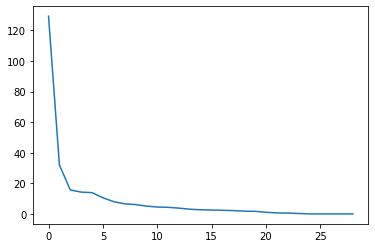
\includegraphics[width=7cm]{svd.png}
  \caption{Spectrum of singular values.}
\end{figure}

The best two and three dimensional representation plot of the data were shown in Figure 2 and 3, respectively. The data appeared to reside in two large clusters. However, there were no obvious linear separation of the event outcomes.

\begin{figure}
\centering
\begin{minipage}{.5\textwidth}
  \centering
  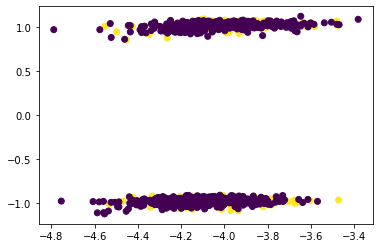
\includegraphics[width=.8\linewidth]{index.png}
  \caption{2-D representation.}
  \label{fig:test1}
\end{minipage}%
\begin{minipage}{.5\textwidth}
  \centering
  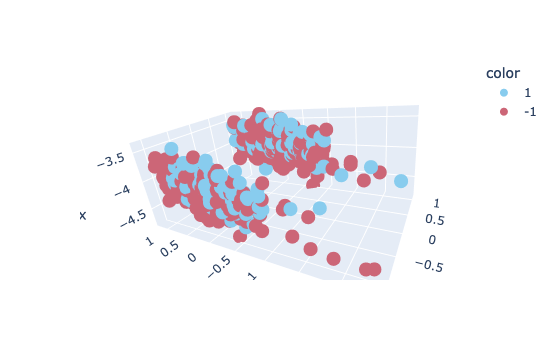
\includegraphics[width=1.1\linewidth]{newplot(8).png}
  \caption{3-D representation.}
  \label{fig:test2}
\end{minipage}
\end{figure}

\subsection{Model Performances}

As previously discussed, ordinary least squares (OLS) model without regularization and with ridge regression were developed as the baseline classification model. As the training data were not in full rank, we utilized the truncated SVD up to the 24th column to make the data full rank.

The OLS model achieved 81.4\% accuracy in training and 80.2\% in testing. On testing, it has 41.4\% recall, 78.5\% precision with 95.5\% specificity. Ridge regularization does not seem to aid much in terms of performance. Best performance on testing were obtained when setting $\lambda = 0.01$, with overall accuracy of 81.4\%, recall rate of 41.5\%, precision of 78.5\% and specificity of 95.5\%. Larger lambda tends to increase specificity while decreases recall. On the other hand, truncated SVD with the first 10 singular values did not perform well both in training and testing, with 72.1\% and 73.6\% overall accuracy respectively.  While both have almost 100\% specificity, both exhibit poor sensitivity of 3.5\% in training and 6.5\% in testing.

Support Vector Machine (SVM) classifier without kernels performs slightly worse, with 76.7\% overall training accuracy and 76.1\% testing accuracy. Of note, it obtained significantly less recall rate of 26.0\%, with specificity of 95.8\%. SVM classifier with the gaussian kernel $k(x_i, x_j) = e^{\frac{-\|xi - xj\|^2}{2 (\gamma)}}$ was developed. It is able to obtain significantly higher training accuracy of 94.4\% (87.1\% recall, 92.6\% precision, 97.2\% specificity), but has lower overall testing accuracy of 72.4\% (56\% recall, 51.1\% precision and 78.9\% specificity), with the highest recall rate on testing set among other models. Classifier with polynomial kernel up to 3 degrees were also developed, but performed poorly over training (50.7\% accuracy) and testing sets (47.9\% accuracy).

\section{Discussion}
\label{discussion}

Dataset used in this project was synthetic data generated with medical record data generation tool. Datasets generated by this tool has been used numerous times, such as for the precisionFDA COVID-19 prediction challenge by the Veteran Health Administration.\cite{VHA} Synthetic dataset has the advantages of preserving privacy of real patients while still providing space for creating predictive models with acceptable accuracy.\cite{foraker} While it might not be representative of real-world health record data, it does provide a realistic view of the overall complexity and is an acceptable compromise to overcome the limited availability of medical data sets due to regulatory restrictions. This project demonstrates the feasibility and possible approach of machine learning given healthcare dataset of this structure. 

The OLS classifier performed quite decently in training and generalize quite well in the testing dataset. On this overdetermined dataset with significantly more examples than features, ridge regularization turned out not to increase model performance. Truncated SVD with reduced rank also did not perform well, particularly in distinguishing positive event (which occurs less often) from negative. This suggests that the distinguishing information of these positive occurences were mostly contained on the remaining features with less variance, which explains why the model struggles in predicting these features and obtain decent sensitivity. 

The overall less number of  observation of the positive events in the dataset might contribute to this fact. This means that increasing the proportion of positive events might be one avenue to increase performance of the model. This problem is common in healthcare, where the events of interest is most likely proportionally lower to that of general population (in fact, healthcare practice generally aim to maintain this proportion of unwanted events, such as disease complication or occurence of disease, low). To overcome this problem, oversampling methods might be utilized.\cite{smote}

We experimented with several different $\gamma$ denumerator parameter on the gaussian kernel. The smaller the $\gamma$ is, we observed that the model tends to converge quickly and performed highly decently on the training data, but did not perform as well on the test set. This suggests the model tends to overfit on the higher-dimensional feature space that the kernel function introduces.

While the dataset used contained reasonably large number of populations, there were only $1,458$ instances ended up being used in this project. For future work, increasing the number of available instances for the model will be a good starting point. In addition, there were more available features in the dataset that have not been incorporated, such as physician billing claims, medical procedures, as well as health care encounters that may potentially contain information to increase performance of the model. However, increasing features should be approached with caution as it won't necessarily always increase performance. In fact, the not full rank nature of the dataset used in this project might suggest that there might be features that can be safely omitted without impacting the model performance. 

\pagebreak

\bibliographystyle{abbrvnat}
\bibliography{cmsc}

\end{document}
